% vim: set textwidth=78 autoindent:

\subsection{Complemento Interpolaci\'on}

% when the revision of a section has been finalized, 
% comment out the following line:
%\updatedisclaimer

El complemento de interporlaci\'on puede ser usado para generar una interpolaci\'on TIN o IDW de una 
capa vectorial de puntos. Es muy simple de manejar y provee una interfaz de usuario gr\'afica 
para crear capas raster de interpolaci\'on (Vea la figura \ref{fig:interpolation_dialog}).
El complemento requiere que los siguientes par\'ametros sean especificados antes de correr:

\begin{itemize}
\item \textbf{Capa vectorial de entrada}: Especifica la capa vectorial de puntos de entrada desde una lista de capas de puntos cargadas.
\item \textbf{Atributo de interpolaci\'on}: Selecciona una columna de atributo a ser usada para interpolaci\'on o 
activa la caja de verificaci\'on \checkbox{Usar coordenada Z} para usar los valores de Z almacenados en las capas.
\item \textbf{M\'etodos de interpolaci\'on}: Selecciona el m\'etodo de interpolaci\'on. Puede ser \selectstring{Triangulated Irregular 
Network (TIN)}{\ldots} o bien \selectstring{Inverse Distance Weighted (IDW)}{\ldots}.
\item \textbf{N\'umero de columnas/filas}: Especifica el n\'umero de filas y columnas para el archivo raster de salida.
\item \textbf{Archivo de salida}: Especifica un nombre para el archivo raster de salida.
\end{itemize}

\begin{figure}[ht]
   \begin{center}
   \caption{Complemento de interpolaci\'on \nixcaption}\label{fig:interpolation_dialog}\smallskip
   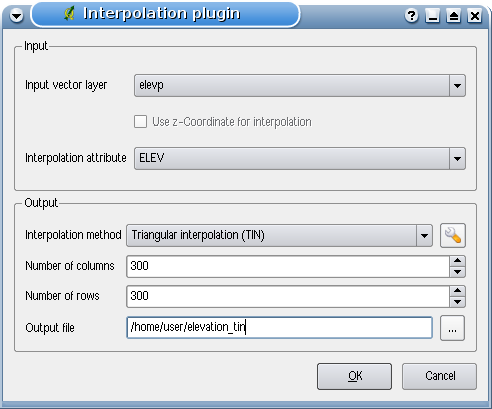
\includegraphics[clip=true, width=9cm]{interpolate_dialog}
\end{center}  
\end{figure}

\minisec{Usando el complemento}\label{interpolation_usage}

\begin{enumerate}
  \item Inicie QGIS y cargue una capa vectorial de puntos (ej., \filename{elevp.csv}). 
  \item Cargue el complemento de interpolaci\'on en el manejador de complementos (vea la secci\'on 
  \ref{sec:load_core_plugin}) y haga clic en el \'{\i}cono \toolbtntwo{interpolation}{Interpolaci\'on} 
  que aparece en la barra de men\'u de QGIS. El di\'alogo de complemento de interpolaci\'on aparece como 
  se muestra en la figura \ref{fig:interpolation_dialog}.
  \item Selecione una capa de entrada (ej., \selectstring{elevp}{\ldots}) y columna para interpolaci\'on (ej. \filename{ELEV}).
  \item Seleccione un m\'etodo de interpolaci\'on (ej. \selectstring{Triangular interpolation}{\ldots}), y especifique 
  el n\'umero de filas y columnas (ej. 3663 columnas y 1964 filas (esto es el equivalente a una resoluci\'on de pixel de 1000 metros))
  as\'{\i} como el nombre del archivo raster de salida (ej., \filename{elevation\_tin}).
  \item Haga clic en \button{Ok}.
  \item Para el ejemplo actual, haga doble clic \filename{elevation\_tin} en la lista de capas para abrir el di\'alogo propiedades de la capa raster 
  y seleccione \selectstring{Pseudocolor}{\ldots} como mapa de color en la pesta\~na \tab{Simbolog\'{\i}a}. Puede  
  definir una nueva tabla de colores como se describe en la secci\'on \ref{label_rasterprop}.
\end{enumerate}

En la figura \ref{fig:interpolation_idw} puede ver el resultado de la interpolaci\'on IDW con resoluci\'on 366 columnas x 196 filas (10 km) 
para \filename{elevp.csv} visualizada usando la tabla de colores pseudocolor. El procesamiento 
solo toma algunos minutos, y cubre la parte norte de Alaska.

\begin{figure}[ht]
   \begin{center}
   \caption{Interpolaci\'on de datos elevp usando el m\'etodo IDW \nixcaption}\label{fig:interpolation_idw}\smallskip
   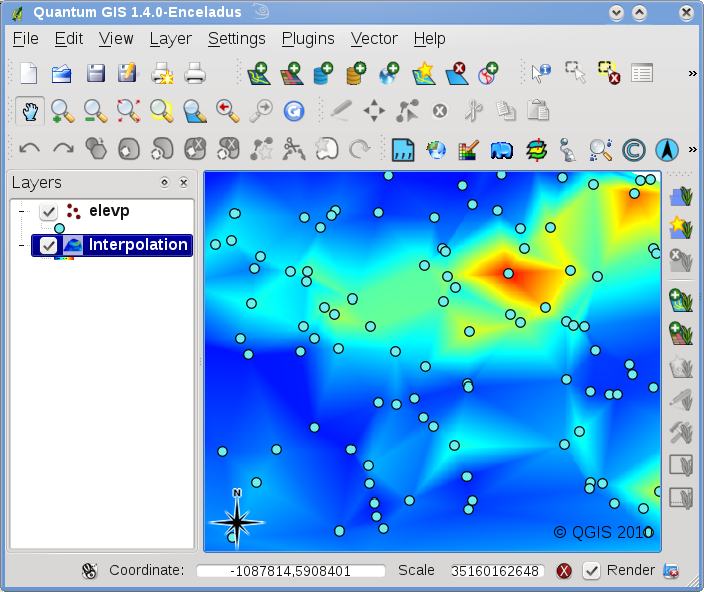
\includegraphics[clip=true, width=12cm]{interpolate_idw}
\end{center}  
\end{figure}

\newpage



